	\subsection{Taxonomy of virtualization technologies by \textit{Kampert}}
	
	\begin{figure}[H]
		\centering
		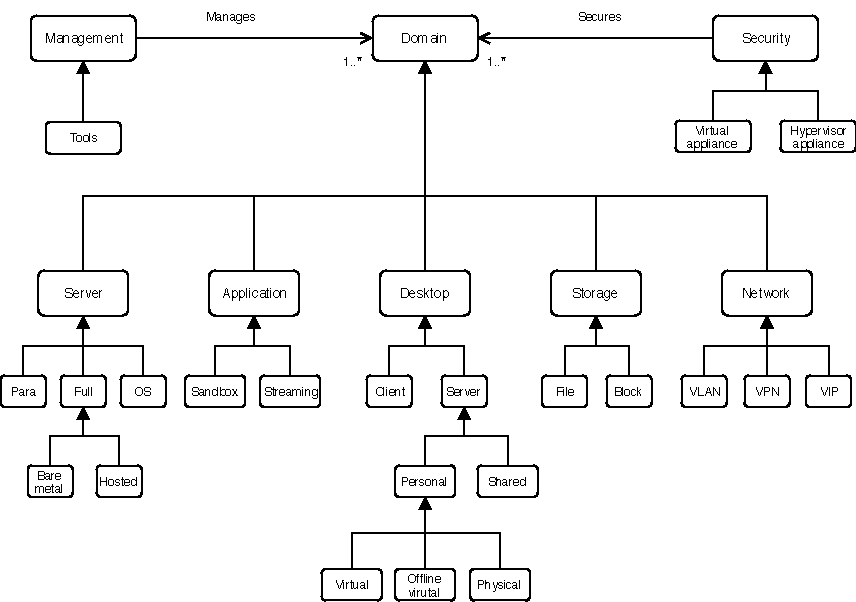
\includegraphics[width=8.5cm]{images/Kampert2010.pdf}
		\vspace{0.2mm}
		\caption{Kampert Taxonomy Model \cite{Kampert2010}.}
		\label{fig:KampertTaxonomyModel2010}
	\end{figure}
	
	In August 2010, \textit {Paulus Kampert} presented his Master's Degree dissertation called \textit{A Taxonomy of Virtualization Technologies} \cite{Kampert2010}. The objective of this work was to provide an overview of the different types of virtualization technologies and their trends. As a result, and with the sponsorship of the virtualization provider \textit{Atos Origin}, the taxonomy model developed shows the different layers of virtual server architecture and the virtualization domains in a structured way.
	
	The \textit{Kampert's} study of focused on the design of a taxonomy model to allow for the illustration of the different virtualization domains and their relationships. This model has been expressed using the Unified Modeling Language (UML), as shown in the Figure \ref{fig:KampertTaxonomyModel2010}.
	
	All elements of the model are called classes. \textit{Domain} is a superclass of the five domain classes: \textit{Server}, \textit{Application}, \textit{Desktop}, \textit {Storage} and \textit {Network}. The superclass in the center of the model facilitates the connection of the domain classes,
	these are \textit{Security} and \textit {Management}. These classes must apply to one or more virtualization domains. Additionally, each model's class can divide into a set of technologies. Below, each class is briefly described:

	\textbf{Server}:  Server virtualization can be divided into three subclasses such as \textit{Para-virtualization}, \textit{Full virtualization} and \textit{OS partitioning}. In turn, the \textit{Full virtualization} is divided into two more subclasses: \textit{Bare-metal} referring to \textit {Type-1 hypervisor} and \textit{Hosted} referring to \textit {Type-2 hypervisor}.
		
	\textbf {Application}: This domain comprises two subclasses corresponding to two types of application virtualization technologies: \textit{Sandbox} and \textit{Application Streaming}.
		
	\textbf{Desktop Virtualization}: Includes two types such as \textit{Client} and \textit{Server}. The \textit{Client desktop virtualization} is used to host virtual desktops (or VMs) on the client's computers. On the other hand, \textit{Server desktop virtualization} is divided into two types: \textit{Personal} and \textit{Shared}. \textit{Personal} is divided into \textit{Virtual}, \textit{Physical} and \textit{Offline virtual}.
		
	\textbf {Storage Virtualization}: Described as the data pool of multiple storage devices. This virtualization is divided into two classes,  \textit {Block virtualization} and \textit {File virtualization}. Examples of these technologies are SAN (\textit{Storage Area Network}) and NAS (Network Attached Storage).
		
	\textbf{Network Virtualization}: This domain comprises three types of technologies; such as, VLAN (LAN virtual), VIP (IP virtual) y VPN (Virtual Private Network).
		
    \textbf{Management}: Includes the five following technologies;  \textit{Performance}, \textit{Configuration}, \textit{Assets}, \textit{Capability} and \textit {Cost-control}.
		
	\textbf {Security}: Refers to the set of technologies developed specifically for virtualization. There are two types: \textit{Hypervisor appliance} and \textit{Virtual appliance}.
		
	\textit{Kampert}'s model intends to cover the domains in a more complete way in which the concept of virtualization takes place. The model itself does not offer the level of granularity necessary to identify particular types and technologies in each of the specified domains.
